\documentclass[Main.tex]{subfiles}
\begin{document}
\section{Variations and Alternative Graphical Methods}
In this section, we will look at some variations and enhancements of the Bland-Altman plot, as well as some alternative graphcial techniques. Strictly speaking, the Identity Plot is advised by Bland and Altman as a prior analysis to the Bland-Alman plot, and therefore is neither a variant nor an alternative approach. However it is worth mentioning, as it is a simple, powerful and elegant technique that is often overlooked in method comparison studies. The identity plot is a simple scatter-plot approach of measurements for both methods on either axis, with the line of equality (the $X=Y$ line, i.e. the 45 degree line through the origin). This plot can gives the analyst a cursory examination of how well the measurement methods agree. In the case of good agreement, the covariates of the plot accord closely with the line of equality.

	\subsection{The Bland Altman Plot - Variations}
	Variations of the Bland Altman plot is the use of ratios, in the
	place of differences.
	\begin{equation}
	D_{i} = X_{i} - Y_{i}   \label{BA01}
	\end{equation}
	Altman and Bland suggest plotting the within subject differences $
	D = X_{1} - X_{2} $ on the ordinate versus the average of $x_{1}$
	and  $x_{2}$ on the abscissa.
	%----------------------------------------------------------------------------%
	
	
\subsection{Variations of the Bland Altman Plot}
\citet{BA99} remarks that it is possible to ignore the issue altogether, but the limits of agreement would wider apart than
necessary when just lower magnitude measurements are considered. Conversely the limits would be too narrow should only higher
magnitude measurements be used. To address the issue, they propose the logarithmic transformation of the data. The plot is then
formulated as the difference of paired log values against their	mean. \citet{BA99} acknowledge that this is not easy to interpret,
and that it is not suitable in all cases.
	
	
	% When selecting this option the differences will be expressed as
	% percentage of the averages. This option is useful when there is an
	% increase in variability of the differences as the magnitude of the
	% measurement increases.
	
		
	% Plot ratios When this option is selected then the ratios of the
	% measurements will be plotted instead of the differences (avoiding
	% the need for log transformation). This option as well is useful
	% when there is an increase in variability of the differences as the
	% magnitude of the measurement increases.
	
%----------------------------------------------------------------------------%


\section{Variations of the Bland-Altman Plot} 
In light of some potential pitfalls associated with the conventional difference plot, a series of alternative formulations for the Bland-Altman approach have been proposed.

Referring to the assumption that bias and variability are constant across the range
of measurements, \citet{BA99} address the case where there is an increase in variability as the magnitude increases. They remark 	that it is possible to ignore the issue altogether, but the limits of agreement would be wider apart than necessary when just lower magnitude measurements are considered. Conversely the limits would be too narrow should only higher magnitude measurements be used. To address the issue, they propose the logarithmic transformation of the data. The plot is then formulated as the difference of paired log values against their mean. Bland and Altman acknowledge that this is not easy to interpret, and may not be suitable in all cases.

	
\citet{BA99} offers two variations of the Bland-Altman plot that are intended to overcome potential problems that the conventional
plot would inappropriate for. The first variation is a plot of case-wise differences as percentage of averages, and is appropriate when there is an increase in variability of the differences as the magnitude increases. The second variation is a
plot of case-wise ratios as percentage of averages. This will remove the need for $log$ transformation. This approach is useful
when there is an increase in variability of the differences as the magnitude of the measurement increases. \citet{Eksborg} proposed
such a ratio plot, independently of Bland and Altman. \citet{Dewitte} commented on the reception of this article by
saying `Strange to say,this report has been overlooked'.

	
	%	%----------------------------------------------------------------%
	%	\section{Dewitte et al }
	%	\begin{quote}When the standard deviation increases with concentration, Bland and Altman recommend a logarithmic y scale, whereas others propose a percent y scale (Pollock et al, 2002). Although generally there is not much difference in effect between using percentages and using a log transformation of the data, we prefer the percent plot (except when data extend over several orders of magnitude) because numbers can be read directly from the plot without the need for back-transformation.
	%	\end{quote}
	%	
	%	\begin{verbatim}
	%	absolute - small range
	%	percentage - medium range
	%	log scale - large range
	%	\end{verbatim}
	%==================================================== %
	
\subsubsection{Bartko's Ellipse}
	
As an enhancement on the Bland Altman Plot, \citet{Bartko} has expounded a confidence ellipse for the covariates. \citet{Bartko} proposes
a bivariate confidence ellipse as a boundary for dispersion. The stated purpose is to `amplify dispersion', which presumably is for  the purposes of outlier detection. The orientation of the the ellipse is key to interpreting the results. The minor axis is related to the between-item variability whereas the major axis is related to the mean squared error (referred to here as Error Mean Square).The ellipse illustrates the size of both relative to each other. 
	
	
Consequently Bartko's ellipse provides a visual aid to determining the relationship between variances. Furthermore, the ellipse provides a visual aid to determining the relationship	between the variance of the means $Var(a_{i})$ and the variance of the differences $Var(d_{i})$. If $\mbox{var}(a)$ is greater than $\mbox{var}(d)$, the orientation of the ellipse is horizontal. Conversely if $\mbox{var}(a)$ is less than $\mbox{var}(d)$, the orientation of the ellipse is vertical. The more horizontal the ellipse, the greater the degree of agreement between the two methods being tested.
	
    %(Furthermore \citet{Bartko}
	%proposes formal testing procedures, that shall be discussed in due
	%course.)
Bartko states that the ellipse can, inter alia, be used to detect the presence of outliers (furthermore \citet{Bartko} proposes formal testing procedures, that shall be discussed in due course). The Bland-Altman plot for the Grubbs data, complemented by Bartko's ellipse, is depicted in Figure ~\ref{GrubbsBartko1}. The fourth observation is shown to be outside the bounds of the ellipse, indicating that it is a potential outlier.
	
	
	\begin{centering}
		\begin{figure}[h!]
			% Requires \usepackage{graphicx}
			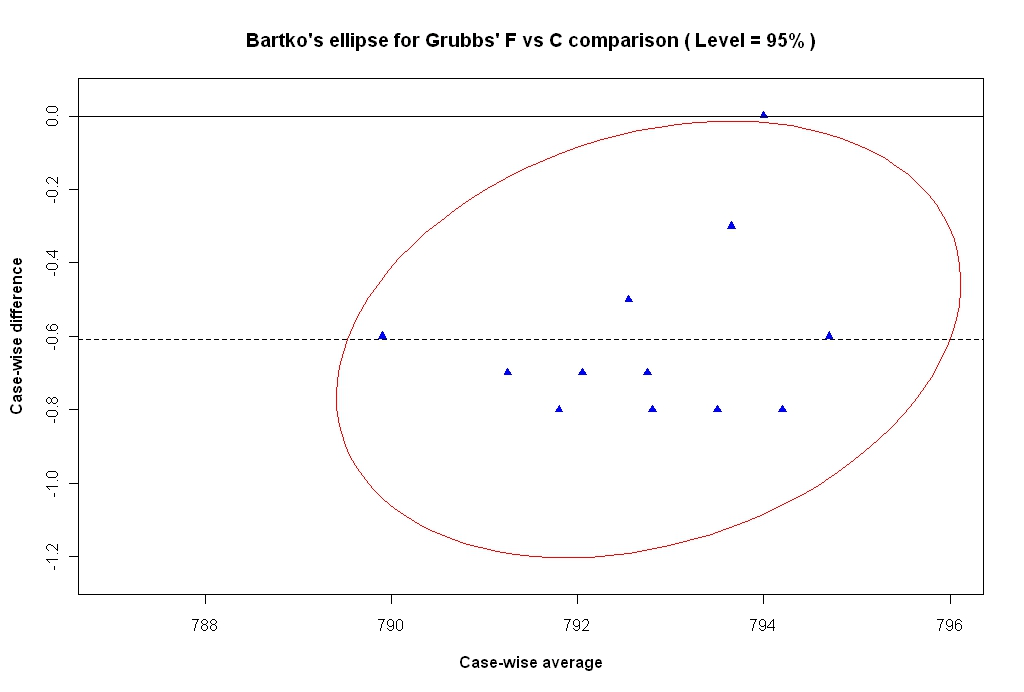
\includegraphics[width=130mm]{images/GrubbsBartko.jpeg}
			\caption{Bartko's Ellipse For Grubbs' Data.}
			\label{GrubbsBartko1}
		\end{figure}
	\end{centering}
	
The limitations of using bivariate approaches to outlier detection in the Bland-Altman plot can demonstrated using Bartko's ellipse. A covariate is added to the `F vs C' comparison that has a difference value equal to the inter-method bias, and an average 	value that markedly deviates from the rest of the average values in the comparison, i.e. 786. Table 1.8 depicts a $95\%$ confidence ellipse for this manipulated data set. By inspection of the confidence interval, a conclusion would be reached that this extra covariate is an outlier, in spite of the fact that this
observation is wholly consistent with the conclusion of the	Bland-Altman plot.
	
	%\begin{figure}[h!]
	%  % Requires \usepackage{graphicx}
	%  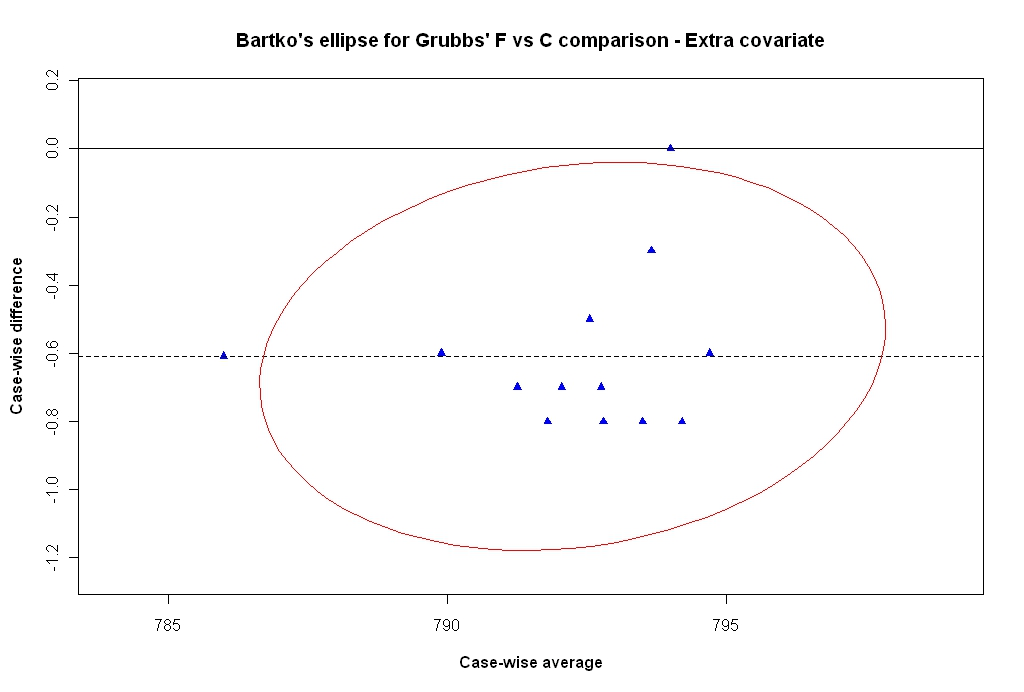
\includegraphics[width=130mm]{images/GrubbsBartko2.jpeg}
	%  \caption{Bartko's Ellipse For Grubbs' Data, with an extra covariate.}\label{GrubbsBartko2}
	%\end{figure}
	
	
Importantly, outlier classification must be informed by the logic of the data's formulation. In the Bland-Altman plot, the horizontal displacement of any observation is supported by two independent measurements. Any observation should not be considered an outlier on the basis of a noticeable horizontal displacement from the main cluster, as in the case with the extra covariate. Conversely, the fourth observation, from the original data set, should be considered an outlier, as it has a noticeable vertical displacement from the rest of the observations.

	
	\begin{figure}[h!]
		% Requires \usepackage{graphicx}
		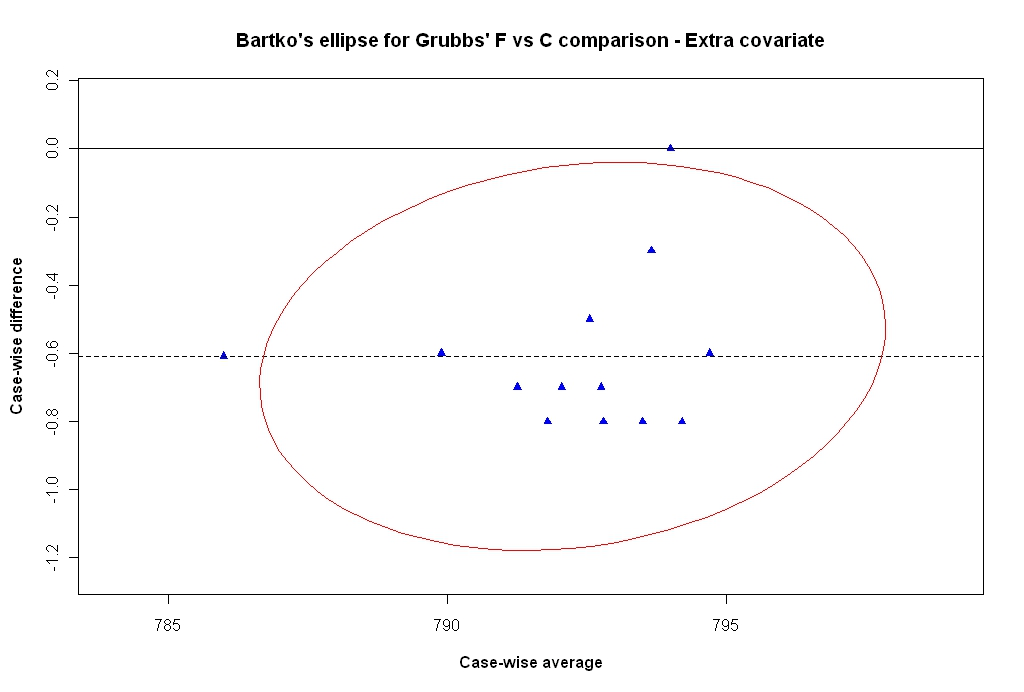
\includegraphics[width=130mm]{images/GrubbsBartko2.jpeg}
		\caption{Bartko's Ellipse For Grubbs' Data, with an extra covariate.}\label{GrubbsBartko2}
	\end{figure}
	
In the Bland-Altman plot, the horizontal displacement of any point on the plot is supported by two independent measurements. Any point should not be considered an outlier on the basis of a noticeable horizontal displacement from the main cluster, as in the case with the extra co-variate. Conversely, the fourth point, from the original data set, should be considered an outlier, as it has a noticeable vertical displacement from the rest of the observations.

	
\subsubsection{Survival-Agreement Plot}
A graphical technique for method comparison studies, that is entirely different to the Bland-Altman plot, was proposed by \citet{luiz}. This approach, known as the survival-agreement plot, is used to determine the degree of agreement using the Kaplan-Meier method, a well known graphical technique in the area of Survival Analysis. Furthermore \citet{luiz} propose that commonly used survival analysis techniques should complement this method,\textit{ providing a new analytical insight for agreement}. Two survival?agreement plots are used to detect the bias between to measurements of the same variable. The presence of inter-method bias is tested with the log-rank test, and its magnitude with Cox regression.
	
	%% TOLERANCE - REWRITE THIS
	
The degree of agreement (or disagreement) of a measure is expressed as a function of several limits of tolerance, using the Kaplan-Meier method, where the failures occur exactly at absolute values of the differences between the two methods of measurement. 
	
According to Luiz et al, the survival-agreement plot is a step function of a typical survival analysis without censored data, where the Y axis represents the proportion of discordant cases. This is equivalent to a step function where the X axis represents the absolute  observed differences and the Y axis is the proportion of the cases with at least the observed difference ($x_i$). 
	
	% % PREVALENCE
	% % Implementation
	
\section*{Mountain Plot}
%% http://www.clinchem.org/content/43/11/2039.long

KW CITE presented a graphical method for evaluation of laboratory assays (a mountain plot). 
They computed the percentile for each ranked difference between the two methods, and by “turning” at the 50th percentile 
produced a histogram-like function (the mountain). 

This method is relevant for detecting large infrequent errors (differences) but lacks the aspect of concentration relationship. 
These investigators, therefore, recommend use of their plot together with difference plots. Introduction of analytical quality specifications in the mountain plots may be useful in method evaluations.

Krouwer and Monti have proposed a folded empirical cumulative distribution plot, otherwise known as a Mountain plot.
	
They argue that it is suitable for detecting large, infrequent errors. This is a non-parametric method that can be used as a complement with the Bland Altman plot.  Mountain plots are created by computing a percentile for each ranked difference between a new method and a reference method. (Folded plots are so called because of the following transformation is performed for all percentiles above 50: percentile = 100 - percentile.) These percentiles are then plotted against the differences between the two methods.
	
Krouwer and Monti argue that the mountain plot offers some following advantages. It is easier to find the central $95\%$ of the data, even when the data are not normally distributed. Also, comparison on different distributions can be performed with ease.
	

\subsection*{Mountain Plot}
A mountain plot (or "folded empirical cumulative distribution plot") is created by computing a percentile for each ranked difference between two methods of measurement.

To get a folded plot, the following transformation is performed for all percentiles above 50: percentile = 100 - percentile. These percentiles are then plotted against the differences between the two methods [Krouwer \& Monti, 1995].

The mountain plot is a useful complementary plot to the Bland \& Altman plot. 
In particular, the mountain plot offers the following advantages:
\begin{itemize}
	\item It is easier to find the central 95% of the data, even when the data are not Normally distributed.
	\item Different distributions can be compared more easily.
	
\end{itemize}
\addcontentsline{toc}{section}{Bibliography}

\bibliographystyle{chicago}
\bibliography{DB-txfrbib}

\end{document} 
